\section{The game}
\label{sec:game}

\subsection{Board and moves}
The board (Fig.~\ref{fig:board}) is the spacetime diagram of the payload: six horizontal wires for the data qubits and one column per layer of CZ gates. A level fixes the depth (6, 12 or 18 layers), the \emph{magic quota} (0, 1, 2, 4, 8 or 16 $T$ gates) and the noise model. The player then makes three decisions, which are precisely the decisions of steps 3 and 6 of the challenge workflow:

\begin{description}[leftmargin=1.2em,itemsep=2pt]
  \item[Post sentinels.] Clicking a qubit label posts a sentinel there: one ancilla that will carry one spacetime check targeting that qubit. The ancilla budget is four. \texttt{add\_pauli\_checks} then decides the Pauli types and the moments at which the check touches its target, and the board draws them as teal probes.
  \item[Inject magic.] The quota of $T$ gates must be placed. After sentinels are posted, every candidate $T$ site is painted green (Z-safe for all checks) or red (covered by an $X$ or $Y$ part of some check flow).
  \item[Choose a placement policy.] \emph{Safe zones} puts the $T$ gates on green sites only, following a fixed random order; if fewer green sites exist than the quota, the move is illegal. \emph{Blind} places them on the first sites of the same order, ignoring the checks. \emph{Blind and retire} uses blind placement but stops post-selecting on any check that the $T$ gates have broken.
\end{description}
\noindent Pressing \emph{Run} reveals the four stages of the pipeline required by the challenge (payload, spacetime checks, ancilla readout, post-selection filter) together with the fidelity without checks $F_0$, the post-selected fidelity $F_{\mathrm{ps}}$, the kept fraction $\kappa$, the cost of the checks (ancillas, extra two-qubit gates, two-qubit depth) and which checks, if any, were broken.

\subsection{Score}
\label{sec:score}
The score is $1000\,R_\beta$ with the \emph{fidelity rate}
\begin{equation}
  R_\beta = F_{\mathrm{ps}}\;\kappa^{\beta}, \qquad 0\le\beta\le1 .
  \label{eq:rate}
\end{equation}
The exponent $\beta$ is the price of a discarded shot and is a slider in the game. Its default value has an operational meaning. Suppose the error left after post-selection damps a traceless observable $O$ by the factor $F_{\mathrm{ps}}$, as a depolarizing residual channel would, and suppose we run $N$ shots and keep $\kappa N$. The estimate of $\langle O\rangle$ obtained by rescaling the post-selected mean by $1/F_{\mathrm{ps}}$ has a standard error of roughly $\sigma_O/(F_{\mathrm{ps}}\sqrt{\kappa N})$, so reaching a precision $\varepsilon$ requires
\begin{equation}
  N \approx \frac{\sigma_O^2}{\varepsilon^2}\,\frac{1}{F_{\mathrm{ps}}^2\,\kappa}=\frac{\sigma_O^2}{\varepsilon^2}\,R_{1/2}^{-2}.
\end{equation}
Hence $R_{1/2}$ is the signal-to-noise ratio per square root of a raw shot, and $R_{1/2}^{-2}$ is the total sampling overhead of detection followed by a rescaling step, which is the detection-plus-mitigation workflow suggested in the \texttt{qiskit-paulice} documentation~\cite{paulice}. Without checks the same argument gives $R=F_0$, so the ratio $G=R_{1/2}/F_0$ tells the player whether the sentinels beat doing nothing. The two extremes are also meaningful: $\beta=0$ rewards purity regardless of cost and $\beta=1$ rewards the yield $F_{\mathrm{ps}}\kappa$, which, for valid checks, can never exceed the fidelity of the unpost-selected checked circuit. A move earns one star if it beats the unprotected circuit, two if it is within 2\% of the best legal move of the level, and three if it is the best.

\subsection{Rule to physics}
Table~\ref{tab:map} lists every rule and the physics it stands for. Two design choices deserve comment. We let \texttt{qiskit-paulice} choose the internal structure of each check rather than letting the player draw controlled-Pauli gates by hand, because a hand-drawn check is almost always invalid and the resulting game would be about bookkeeping rather than about trade-offs. The spatial choice (which qubits carry an ancilla) and the interaction with the $T$ gates remain with the player, and those are the choices that matter. Second, the game keeps the bad options. Blind placement and retiring broken checks are legal because players should discover for themselves, with real numbers, why they are bad.

\begin{table*}[t]
\caption{Game rules and the physics they represent. All quantities are computed with Qiskit; none is hand-set.}
\label{tab:map}
\begin{ruledtabular}
\begin{tabular}{p{0.21\textwidth}p{0.47\textwidth}p{0.26\textwidth}}
Game element & Physics & Computed by \\
\hline
Qubit wire, CZ column & Data qubit, layer of a brickwork Clifford payload & \texttt{QuantumCircuit} \\
Sentinel post (budget 4) & One ancilla and one spacetime check targeting that data qubit & \texttt{add\_pauli\_checks} (\texttt{gamma}, \texttt{windowed}) \\
Teal probes on a wire & Moments at which the check applies a controlled Pauli to its target & checked circuit \\
Syndrome parities at readout & Output bits XORed with the ancilla bit to form the syndrome & \texttt{check\_support} \\
Green / red site & Every check flow acts as $I/Z$ there (T is safe) / some flow acts as $X/Y$ & \texttt{uncovered\_paulis} \\
Magic quota & Number of non-Clifford $T$ gates in the payload & $T$ inserted after check search \\
Safe zones / Blind / Retire & Doping policy; a $T$ on a red site breaks a check (Lemma~\ref{lem:doping}) & noiseless \texttt{Statevector} test \\
Run & Noisy execution with ancilla readout and post-selection & Aer density matrix, exact \\
$F_0$, $F_{\mathrm{ps}}$, $\kappa$ & Fidelity with the ideal state, without and with post-selection; kept fraction & stabilizer or statevector reference \\
Score $1000R_\beta$, stars & Fidelity rate, Eq.~\eqref{eq:rate}; comparison with every legal move & \texttt{sentinels.scoring} \\
\end{tabular}
\end{ruledtabular}
\end{table*}

\subsection{Implementations}
The web version (published with GitHub Pages) is a static page that plays back the Qiskit results for every legal move of every level, so it runs instantly on any device. Each level also shows the full trade-off map of the level, every legal move plotted as $F_{\mathrm{ps}}$ against $\kappa$ with curves of constant $R_\beta$, and reveals the optimum after the player has committed. The terminal version, \texttt{sentinels play}, computes the chosen move live with \texttt{qiskit-paulice} and Qiskit Aer, and a notebook walks through the six steps of the challenge.

\begin{figure*}[t]
\centering
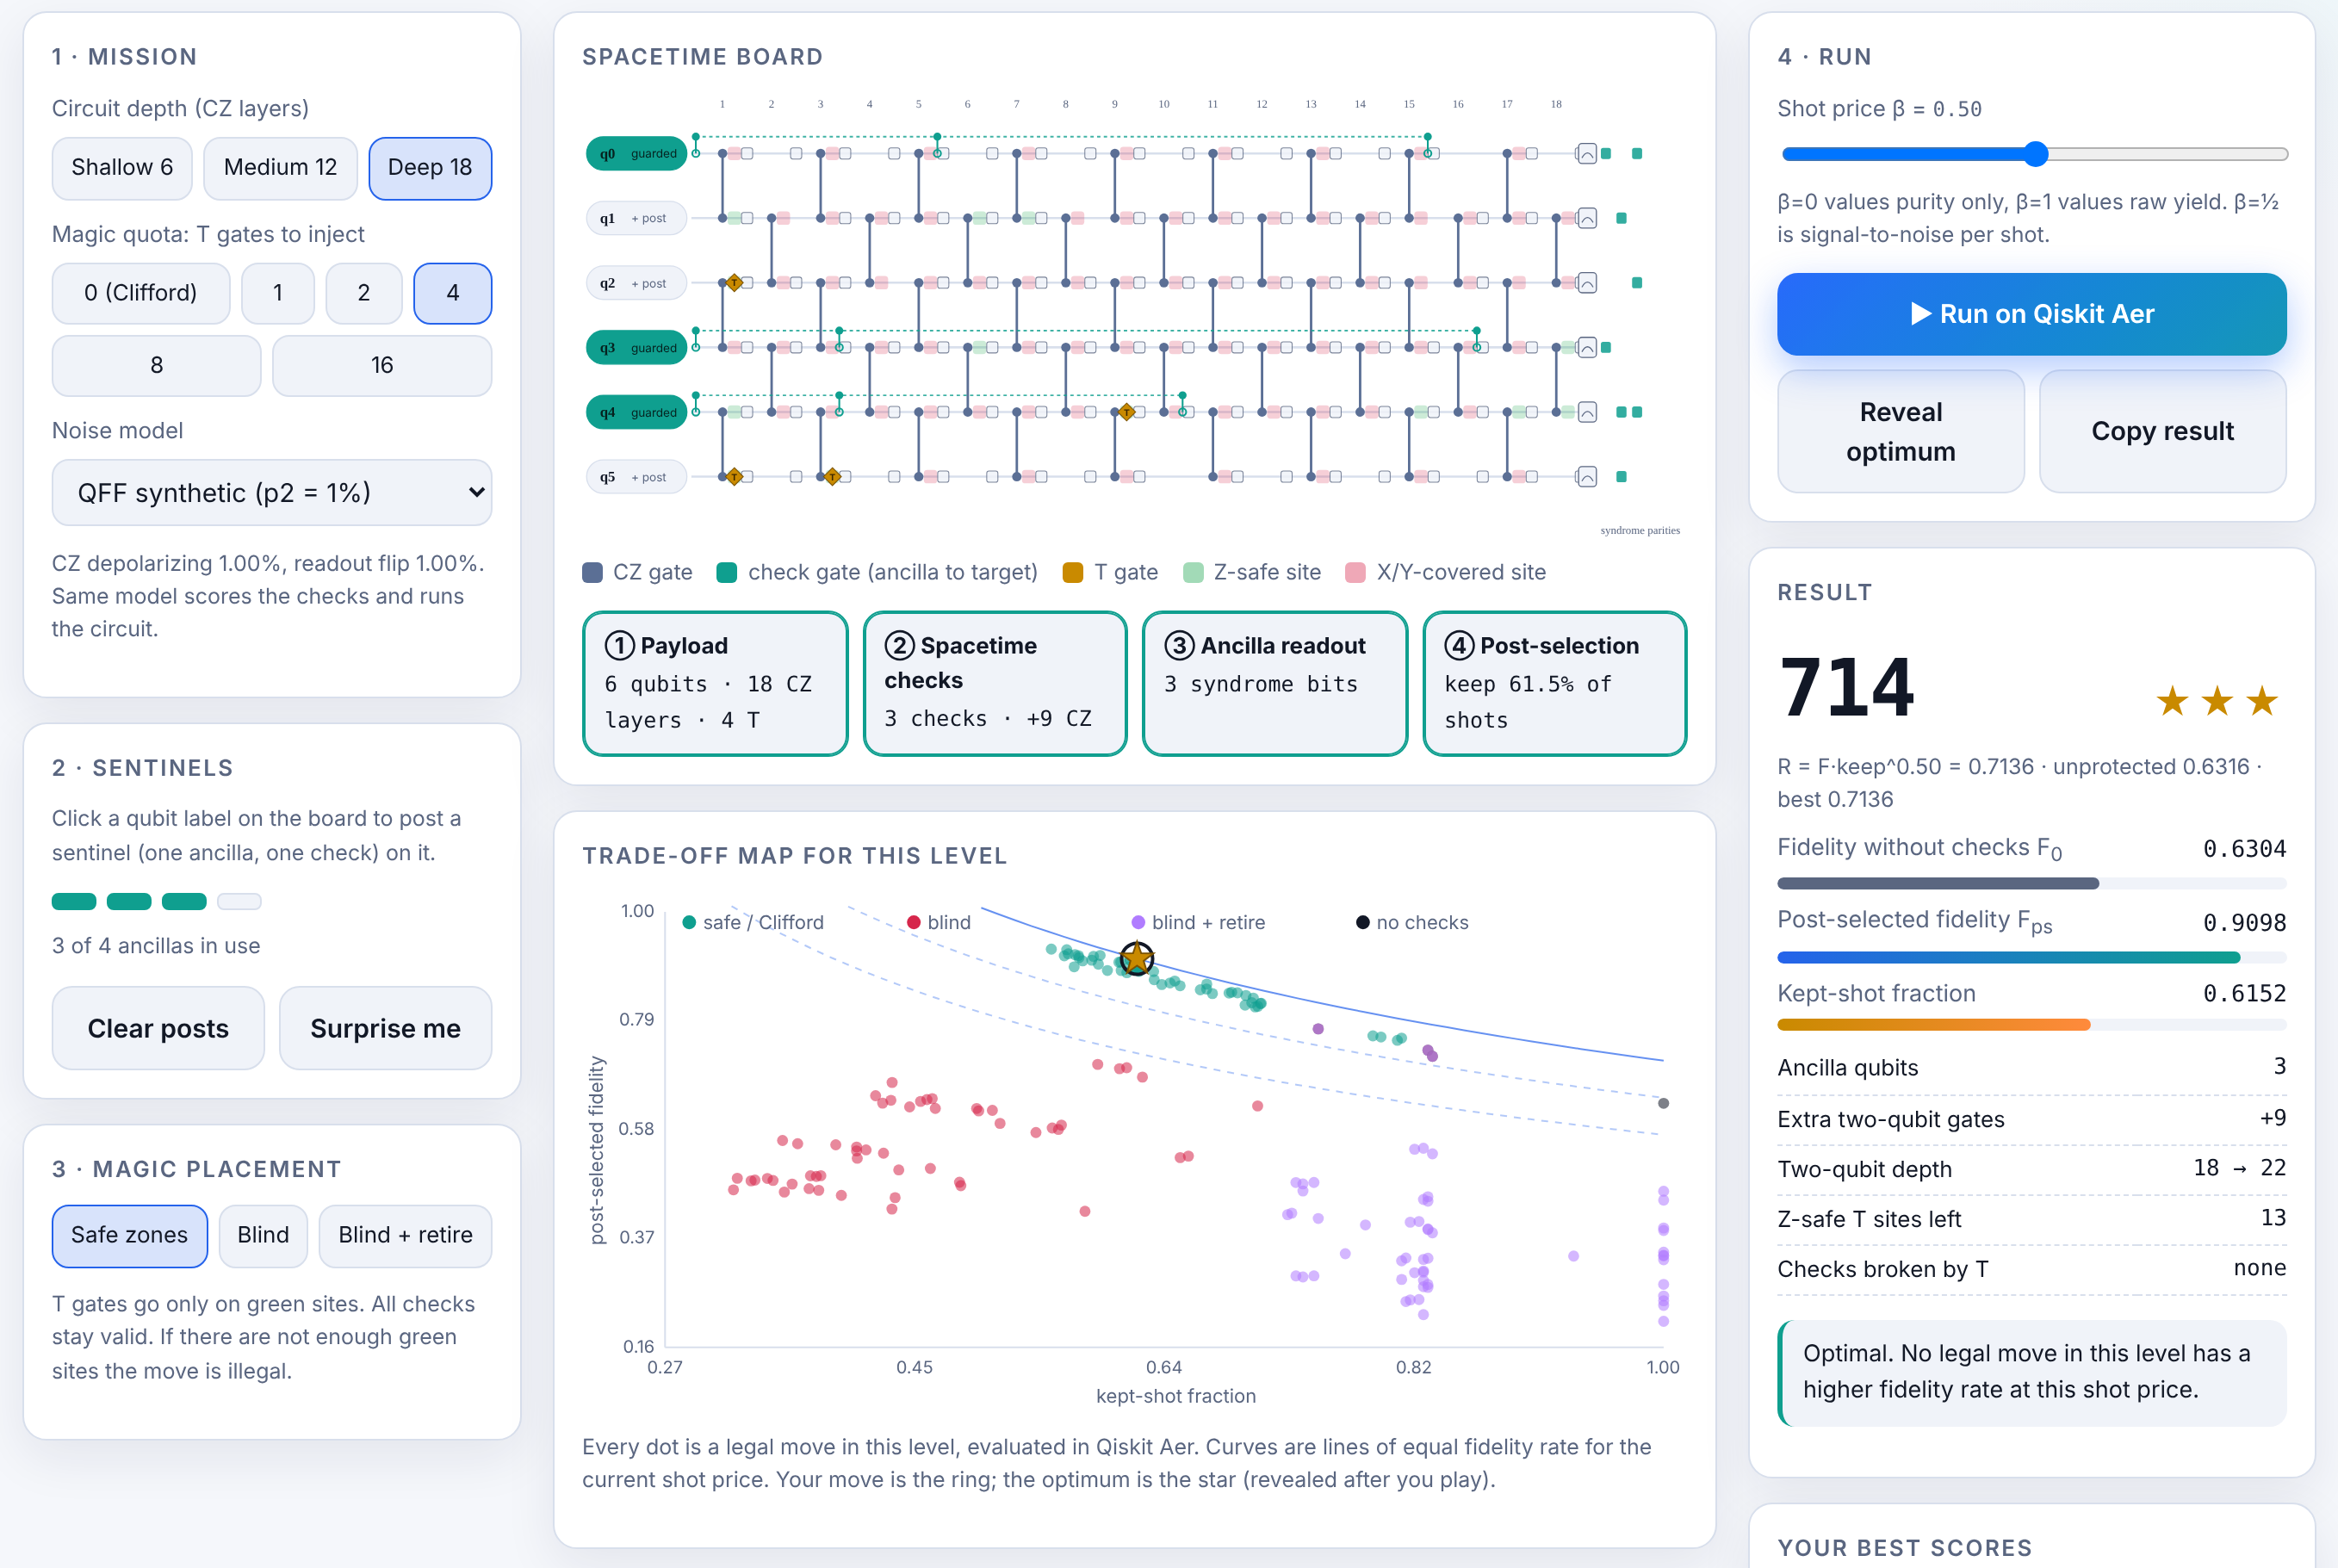
\includegraphics[width=\textwidth]{figures/board.png}
\caption{The web game during a deep level (18 CZ layers, quota of 4 $T$ gates). Sentinels are posted on three qubits; teal probes show where each check touches its target, green and red squares mark Z-safe and covered $T$ sites, gold diamonds are the placed $T$ gates, and the right panel shows the Qiskit result of the move. The lower panel plots every legal move of the level.}
\label{fig:board}
\end{figure*}
